%\documentclass[12pt]{article}
% some macros
%% Here, you can define your own macros. Some examples are given below.

\newcommand{\R}[0]{\mathds{R}} % real numbers
\newcommand{\Z}[0]{\mathds{Z}} % integers
\newcommand{\N}[0]{\mathds{N}} % natural numbers
\newcommand{\C}[0]{\mathds{C}} % complex numbers
\newcommand{\bm}[1]{{\boldsymbol{{#1}}}} % vector
\newcommand{\mat}[1]{{\boldsymbol{{#1}}}} % matrix

\newcommand{\E}[1]{\mathbb{E}_{#1}} % Expectation
\newcommand{\Pd}[1]{\mathbb{P}_{#1}} % Probability Distribution

%%%%%%%%%%%%%%%%%%%%%%%%%%%%%%%%%%%%%%%%%%
% University Assignment Title Page 
% LaTeX Template
% Version 1.0 (27/12/12)
%
% This template has been downloaded from:
%%%%%%%%%%%%%%%%%%%%%%%%%%%%%%%%%%%%%%%%%
%----------------------------------------------------------------------------------------
%	PACKAGES AND OTHER DOCUMENT CONFIGURATIONS
%----------------------------------------------------------------------------------------

\usepackage[nottoc,notlot,notlof]{tocbibind}
\usepackage[T1]{fontenc}
%\usepackage{hyperref}
\usepackage{indentfirst}
\usepackage{amsmath}
\usepackage{amssymb}
\usepackage{graphicx}
\usepackage{subcaption}
\usepackage{geometry}
 \geometry
 {
     a4paper,
     left=25mm,
     right=25mm,
     top=30mm,
     bottom=30mm,
 }

% \usepackage[a4paper,hmargin=2.8cm,vmargin=2.0cm,includeheadfoot]{geometry}
\usepackage{textpos}
\usepackage{natbib} % for bibliography
%\usepackage{tabularx,longtable,multirow,subfigure,caption}
\usepackage{fncylab} %formatting of labels
\usepackage{fancyhdr} % page layout
\usepackage{url} % URLs
\usepackage[english]{babel}
%\usepackage{dsfont}
\usepackage{epstopdf}
\usepackage{backref} % needed for citations
\usepackage{array}
\usepackage{latexsym}
\usepackage[pdftex,pagebackref,hypertexnames=false,colorlinks]{hyperref} % provide links in pdf
 
\hypersetup{pdftitle={},
  pdfsubject={}, 
  pdfauthor={},
  pdfkeywords={}, 
  pdfstartview=FitH,
  pdfpagemode={UseOutlines},% None, FullScreen, UseOutlines
  bookmarksnumbered=true, bookmarksopen=true, colorlinks,
    citecolor=black,%
    filecolor=black,%
    linkcolor=black,%
    urlcolor=black}
 
\usepackage[all]{hypcap}
\frenchspacing

\DeclareMathOperator{\tr}{tr}

%\begin{document}

\section{Facial Mesh Alignment}
In order to create blendshapes from 3D facial scans, movement within scans should be limited to facial movement with as little head movement as possible.
If head movement remains within the scans, then this will be reflected in the principal axis produced by Principle Components Analysis (PCA) and as head motion is independent from speech, this is undesirable.
Initial data capture can aim to minimise subject head movement, however this cannot be completely eliminated.
To remove head motion from the dataset, the scans can be brought into alignment relative to landmark positions on the face which do not move during speech.
Such landmarks include the nose, corners of the eyes and cheek bones, as these points which will be stationary during speech.
By aligning the meshes based on the variation in these points, the head position of the subjects can be constrained while the mouths are not.
To achieve this, Procrustes Analysis can be used.

\subsection{Procrustes Analysis} \label{sec:procrustes_analysis}
Procrustes Analysis is a statistical shape analysis method used to analyse the differences between two objects \cite{Krzanowski2000}.
Given matrices $\mat{X} \in \mathbb{R}^{(n\times f)}$ and $\mat{Y} \in \mathbb{R}^{(n\times f)}$, each representing the coordinates of $n$ points in an $f$-dimensional feature space, a common statistical difference metric is the sum of square differences (\ref{eq:ssd}).
\begin{equation}
    \label{eq:ssd}
    D = \sum_{i=1}^{n} \sum_{j=1}^{f} (x_{ij} - y_{ij})^2
\end{equation}

\noindent However, two objects which are mathematically similar can still have a significant difference when they are scaled differently and are in different positions, orientations in space.
In order to compare two objects regardless of these factors, the differences in orientation, scale and spacial position of the objects must be minimised by bringing the objects into optimal alignment.

\subsubsection{Translational Alignment} \label{sec:trans_align}
Translational components can be eliminated by having the centroids of the two objects lie at the same position in space.
This can be easily achieved by subtracting the mean of each objects points from itself such that the centroid now lies at the origin.

Let $\bar{x}_j = \frac{1}{n} \sum_{i=1}^{n} x_{ij}$ and $\bar{y}_j = \frac{1}{n} \sum_{i=1}^{n} y_{ij}$ where $(j = 1, \dots, f)$ represent the mean of each feature, such that the centroids of the two objects are given by $C_X = (\bar{x}_1, \bar{x}_2, \dots, \bar{x}_f)$ and $C_Y = (\bar{y}_1, \bar{y}_2, \dots, \bar{y}_f)$ respectively.
By subtracting the mean of $\mat{X}$ and $\mat{Y}$ from themselves, the centroids $C_X$ and $C_Y$ will be in alignment at the origin, minimising the sum of square differences due to translational components.

\subsubsection{Scaling Alignment} \label{sec:scale_align}
Similarly, scaling components can be removed by rescaling the objects by the root mean square distance (\ref{eq:rms}), such that the root mean square distance will be of unit distance for both.

\begin{equation}
    \label{eq:rms}
    D = \sqrt{\frac{1}{n} \sum_{i=1}^{n} \sum_{j=1}^{f} x_{ij}^2}
\end{equation}

\subsubsection{Rotational Alignment} \label{sec:rot_align}
In order to align the objects in the same orientation, a rotational matrix which is able to map $\mat{X}$ to $\mat{Y}$ as closely as possible must be found.
This is described as the Orthogonal Procrustes problem and can be solved with Singular Value Decomposition (SVD).
Given matrices $\mat{A}$ and $\mat{B}$, the orthogonal matrix $\mat{R}$ is the matrix which matches $\mat{A}$ to $\mat{B}$ as closely as possible, as described by equation (\ref{eq:orth_proc_prob}), where $\| \cdot \|_F$ is the Fobius norm.

\begin{equation}
    \label{eq:orth_proc_prob}
    \mat{R} =\operatorname*{arg}\operatorname*{min}_\mat{\Omega} 
        \| \mat{\Omega} \mat{A} - \mat{B} \|_F
        \quad
        \text{subject to}
        \quad
        \mat{\Omega}^\top \mat{\Omega} = \mat{I}
\end{equation}

\noindent
The product of matrices $\mat{A}$ and $\mat{B}$ can be decomposed (\ref{eq:svd_2}), and then the rotational matrix $\mat{R}$ can be expressed (\ref{eq:proc_rotation}).
\begin{equation} \label{eq:svd_1}
    \mat{M} = \mat{B} \mat{A}^\top
\end{equation}
\begin{equation} \label{eq:svd_2}
    \mat{M} = \mat{U} \mat{\Sigma} \mat{V}^\top
\end{equation}
\begin{equation} \label{eq:proc_rotation}
    \mat{R} = \mat{U} \mat{V}^\top
\end{equation}

\subsubsection{A Simple Application of Procrustes Analysis}
This section follows the steps of object alignment using Procrustes Analysis as described above with a simple example.
A pair of configurations are given by the matrices below, visualised in Figure \ref{fig:procrustes_ex_1}.

\begin{equation*}
    \mat{X} = 
    \begin{pmatrix} 
        1 & 1 \\
        1 & 2 \\
        3 & 2
    \end{pmatrix}
    \quad 
    \text{and} 
    \quad 
    \mat{Y}
    \begin{pmatrix} 
        -3 & -2 \\
        -3 & -4 \\
        -7 & -4
    \end{pmatrix}
\end{equation*}

\begin{figure*}[t]
    \centering
    \begin{subfigure}[b]{0.475\textwidth}
        \centering
        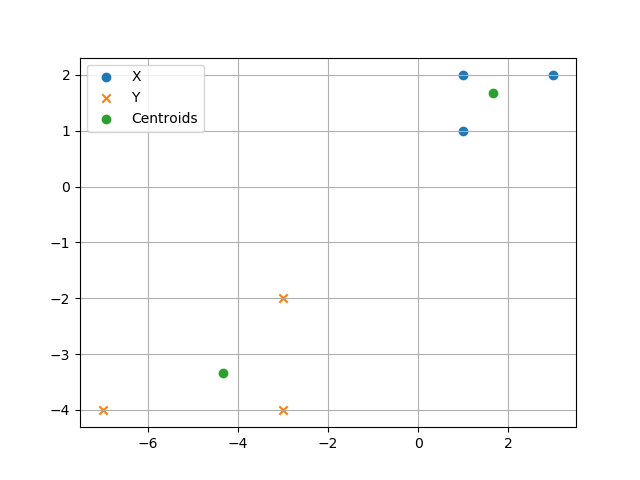
\includegraphics[width=\textwidth]{figures/procrustes_ex1}
        \caption[]
        {{\small Original coordinates}}    
        \label{fig:procrustes_ex_1}
    \end{subfigure}
    \begin{subfigure}[b]{0.475\textwidth}  
        \centering 
        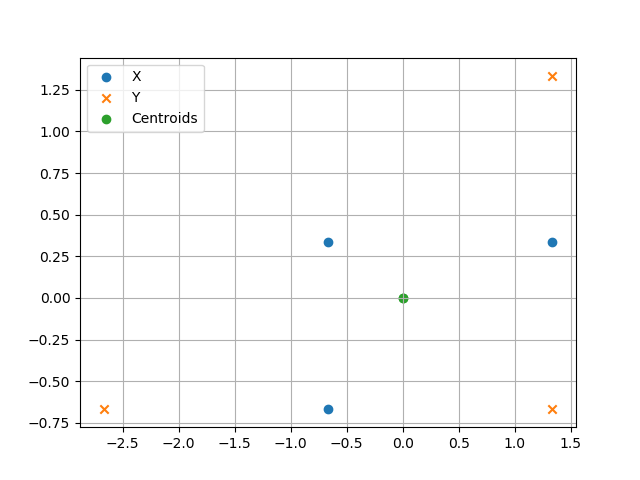
\includegraphics[width=\textwidth]{figures/procrustes_ex2}
        \caption[]
        {{\small Translation}}    
        \label{fig:procrustes_ex_2}
    \end{subfigure}
    \begin{subfigure}[b]{0.475\textwidth}   
        \centering 
        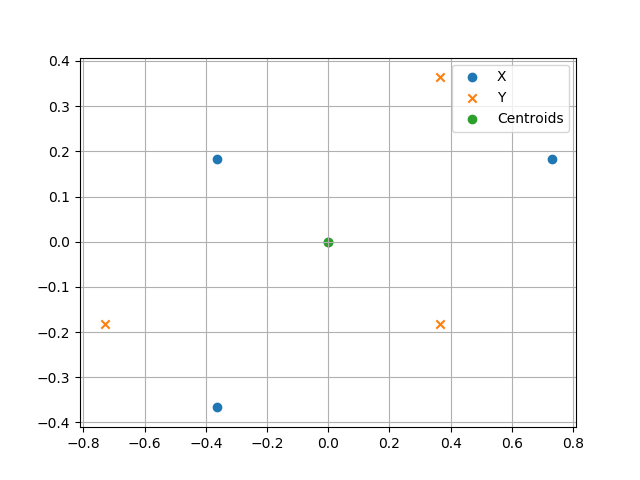
\includegraphics[width=\textwidth]{figures/procrustes_ex3}
        \caption[]
        {{\small Scaling}}    
        \label{fig:procrustes_ex_3}
    \end{subfigure}
    \begin{subfigure}[b]{0.475\textwidth}   
        \centering 
        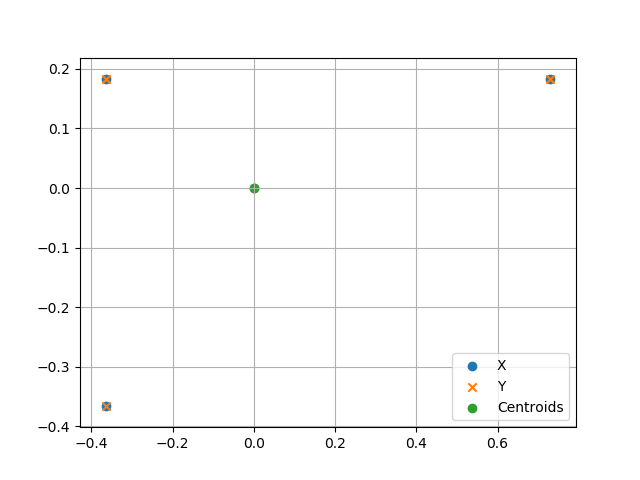
\includegraphics[width=\textwidth]{figures/procrustes_ex4}
        \caption[]
        {{\small Rotation}}    
        \label{fig:procrustes_ex_4}
    \end{subfigure}
    \caption[]
    {Application of Procrustes Analysis} 
    \label{fig:procrustes_analysis}
\end{figure*}


\noindent
Before applying alignment, the sum of square differences between $\mat{X}$ and $\mat{Y}$ is
\begin{align*}
    D& = {(1+3)^2 + (1+2)^2} + {(1+3)^2 + (2+4)^2} + {(3+7)^2 + (2+4)^2} \\
     & = 213
\end{align*}
As described in section (\ref{sec:trans_align}), the initial objects are translated so that their centroids lie at the origin (Figure \ref{fig:procrustes_ex_2}). This is then followed by scaling alignment and finally rotational alignment (Figures \ref{fig:procrustes_ex_3}, \ref{fig:procrustes_ex_4}).
After alignment, the difference is zero as these objects are both similar triangles.

\subsection{Procrustes Analysis for Facial Mesh Alignment}
The process of Procrustes Analysis described above deals with objects in which all coordinate points are used to find the optimum alignment, however this is inappropriate for facial mesh alignment as not only would the position of the head be aligned to, but as would the motion from speech, of which the aim is to maintain variation.
However, a subset of points of a pair of objects can be used to align the entire object.
By selecting points which do not contain any movement due to speech or facial expression, variation in these points can be assumed to be only from head motion.
Such positions include the nose, corners of the eyes and cheekbones.
If the facial scans capture 360 degrees, then points on the back of the subjects head can also be used.
From this subset of points, the translation, scaling and rotational matrix can be found which aligns these points using the steps described in section \ref{sec:procrustes_analysis} but then applied to the entire object.
    
%\newpage
%\bibliographystyle{unsrt}
%\bibliography{ref}
%\end{document}